% !Mode:: "TeX:UTF-8"
\chapter{Transfert thermique}
\section{Des nombres importants}
Biot:$$B_i = \frac{ hD}{\lambda }=\frac{\tau^{cd}}{\tau^{cc}}$$
$$B_i = \frac{ \text{coefficient de transfert } \times \text{dimension caract\'eristique} }{\text{conductivit\'e thermique}}$$
Comme $$Re=\frac{U\times l}{\nu}$$
$U$: la vitess de fluide(transfert)\\
$\nu$: coefficient de viscosit\'e dynamique\\
Il qui caract\'erise le r\'egime d'\'ecoulement

Diffusivit\'e thermique $a$ en $m^2/s$:$$a=\frac{\lambda }{\rho c_p};\frac{\partial T}{\partial t}=a\triangle T + \frac{P}{\rho c_p}$$

Nombre de Fourier:$$F_0=\frac{ at}{x^2}$$

Le temps caract\'eristique de conduction thermique:$$\tau^{cd}=\frac{x^2}{a}$$
Le temps caract\'eristique de convection thermique:$$\tau^{cc}=\frac{\tau^{cd}}{B_i}=\frac{e^2/a }{he/\lambda }=\frac{\rho c_p e}{h}$$

La longueur caract\'eristique de conduction thermique \`a l'instant $t$:$$l^{cd}=\sqrt{at}$$

Effusivit\'e thermique du mat\'eriau:$$b=\sqrt{\lambda \rho c}$$
il caract\'erise sa capacit\'e \`a \'echanger de l'\'energie thermique avec son environnement\\

La profondeur de p\'en'etration $e_p$:$$e_p=\sqrt{\frac{2a}{\omega}}$$
透射率(当透射率小于某一个值时,可以认为ne passe pas):$$\tau = exp(-\frac{x}{e_p})$$


流体的温度-$x$变化曲线的横截距,式中$\lambda$为fluide的参数:$$\eta=\frac{\lambda }{h}$$

\subsection{Convection forc\'ee}
le nombre de Nusselt:$$N_u = \frac{hD}{\lambda }=\frac{D/\lambda }{1/h}=\frac{R^{cd}}{R^{cc}}=A\cdot (R_e)^{\alpha}\cdot (P_r)^{\beta}$$
C'est donc le rapport de la r\'esistance thermique de conduction par la r\'esistance thermique de convection. Il est d'autant plus \'elev\'e que la convection est pr\'edominante sur la conduction. Il caract\'erise le type de transfert
de chaleur.\\
\textbf{Propri\'et\'es thermophysiques du fluide $\rho, \mu, \nu, C_p, \lambda, a$ sont \'evalu\'es \`a la temp\'erature de film $T_f = (T_0 + T_p)/2$}

Le nombre de Prandtl:
$$
P_r = \frac{ \mu C_p}{\lambda }=\frac{ \nu}{a}
$$
$$
\frac{\text{Diffusivit\'e de quantit\'e de mouvement $\nu$ (ou viscosit\'e cin\'ematique)}}{\text{Diffusivit\'e thermique}}
$$
对于常见的流体:
\begin{description}
\item [Fluides ususels:] $P_r$ de l'ordre $1$
\item [M\'etaux liquides:] $P_r$ de l'ordre $10^{-2}$ 说明液态金属的传热性能非常好
\item [Huiles:] $P_r$ de l'ordre $10^3$
\end{description}

Le nombre de P\'eclet:$$P_e = R_e \cdot P_r$$

\subsubsection{Convection forc\'ee externe laminaire}
\begin{eqnarray}
 0.6<P_r<10 & \frac{ \delta _{th}}{\delta _m}=pr^{-1/3} \\
 & h(x)=\frac{ \lambda }{\frac{ 2}{3}\delta _{th}(x)}
\end{eqnarray}

\subsection{Convection naturelle}
Le nombre de Grashof(comme nombre de Reynolds):
$$G_{r_L} = \frac{ \rho^2 g \beta (T_p - T_0)L^3}{\mu ^2}$$
$$N_{u_L} = C G_{r_L}^{\alpha}P_r^{\beta}$$
$$G_{r_x} = \frac{ \rho^2 g \beta (T_p - T_0)x^3}{\mu ^2}$$
$$N_{u_x} = C^{\prime} G_{r_x}^{\alpha}P_r^{\beta}$$

\begin{itemize}
\item $G_{r_x}\leq 10^9$ laminaire
\item $G_{r_x}\geq 10^9$ et $G_{r_x} \leq 10^{10}$ transitoire
\item $G_{r_x}\geq 10^{10}$ turbulent
\end{itemize}

Le nombre de Rayleigh:\\
Nombre de Rayleigh fait intervenir le terme moteur(Archim\`ede) et les deux ph\'enom\`enes de diffusion:le frottement visqueux $\nu$ mais aussi la conduction thermique $a$, ce qui est plus physique.
$$R_{a_x}(x)=G_{r_x}P_r=\frac{ g\beta(T_p - T_0)x^3}{\nu a}$$
$$N_{u_L} = C R_{a_L}^{\alpha'}P_r^{\beta'}$$
$$N_{u_x} = C^{\prime} R_{a_x}^{\alpha'}P_r^{\beta'}$$
Ces r\'esultats sont faiblement d\'ependants du nombre de Prandtl.

\subsection{Massique}
\begin{tabular}{|c|c|}
\hline
transfert de chaleur & transfert d'esp\`ece \\
\hline
$\varphi^{cc}= - \lambda \vec{\mbox{grad}}T$ & $q^{cc}= - D_{s/m} \vec{\mbox{grad}}c $\\
\hline
$\varphi^{cc}=h^{cc}(T_p - T_f)$ & $q^{cc}=h^{cc}(c_p - c)$\\
\hline
$h^{cc}$ coefficient de transfert conducto-convectif ($Wm^{-2}K^{-1}$) & $h^{cc} $($m/s$) \\
\hline
$R_{e_x}=\frac{ux}{\nu}$ et $R_{e_L}=\frac{ uL}{\nu}$ & $R_{e_x}=\frac{ux}{\nu}$ et $R_{e_L}=\frac{ uL}{\nu}$ \\
\hline
$P_r=\frac{ \nu}{a} $& $S_c=\frac{\nu}{D_{s/m}} $\\
\hline
$N_u$ & $S_h $\\
\hline
$\frac{ dH}{dt}=\varphi S$ & $\frac{dM}{dt}=qS$\\
\hline
\end{tabular}

Le changement d'enthalpie: $$dH=m c_p dT \quad (J)$$
En r\'egime stationnaire pour gaz parfait ou liquide
$$\frac{ dH}{dt}=\dot{m}c_p dT_m$$


%--------------------------------------------------------------------------%
%--------------------------------------------------------------------------%
\section{Mod\`ele}
\subsection{Ailette:$B_i < 0.1$}
pour une barre de section carr\'ee a et de longeur L:
对于一般图形来说,没有一个确定的量能够单独表示特征尺寸,所以一般用$\frac{\text{面积}}{\text{周长}}$来表示这个特征尺寸
\begin{eqnarray}
\text{sa longeeur caract\'eristique}\quad l=\frac{A}{P}=\frac{a^2}{4a} \\
B_i = \frac{ hl}{\lambda }
m=\sqrt{\frac{ h}{l\lambda }}=\sqrt{\frac{ hP}{\lambda A}} \\
\end{eqnarray}
\subsubsection{Ailette id\'eale}
$$
m\cdot l \leq 1 \quad \frac{T(z)-T_f}{T_p - T_f} \simeq 1
$$
La temp\'erature de l'ailette rest en tout point tr\`es voisine de $T_p  \Rightarrow \frac{ T - T_f}{T_p - T_f}\simeq 1$
\subsubsection{Ailette infinie}
$$
m\cdot l \geq 3 \quad  \frac{T(z)-T_f}{T_p - T_f}=exp(-mz)
$$
Aucun flux n'est plus dissip\'e en bout d'ailette. En effet, au bout d'une certaine longueur, la temp\'erature de l'ailette est proche de la temp\'erature de r\'ef\'erence du fluide.Le flux \'echang\'e tend vers $0$.

\subsubsection{D\'emonstration}
%\begin{figure}
%\def\svgwidth{0.5\columnwidth}
%\input{image/ailette.pdf_tex}
%\end{figure}

\begin{eqnarray}
 \text{en z:} & \Phi_1=\varphi(z)\cdot A \\
 \text{en z+dz:} &\Phi_2=-\varphi(z+dz) \cdot A\\
 \text{en surface lat\'eral:} & \Phi_3=-h(t(z)-T_f) \cdot P_m dz \\
 \text{三个flux相加为零(考虑了进出的符号问题):}  &\Phi_1 + \Phi_2 + \Phi_3 = 0
 \end{eqnarray}

\begin{eqnarray}
 \text{en z:} & \Phi_1=- \lambda \frac{dT}{dz} \cdot A \\
 \text{en z+dz:} &\Phi_2=-\lambda \frac{ d}{dz}(T+\frac{dT}{dz}dz) \cdot A\\
 \text{en surface lat\'eral:} & \Phi_3=h(T(z)-T_f) \cdot P_m dz \\
 \text{三个flux都为正值,但是$\Phi_1$进去,$\Phi_2,\Phi_3$都是出去:}  &\Phi_1 - \Phi_2 - \Phi_3 = 0\\
\end{eqnarray}

R\'esultat:
\begin{equation}
	\begin{split}
	\frac{ d^2T}{dz^2}=\frac{ hP_m}{\lambda A}(T(z)-T_f)=m^2(T(z)-T_f) \\
	 T-T_f=A e^{mz} + B e^{-mz}
	\end{split}
\end{equation}
Pour l'ailette infinie
\begin{equation}
	\begin{split}
	  \text{温度不能无穷大}\Rightarrow A=0 \\
	  \text{en} z=0 \quad T_p - T_f =B \Rightarrow \frac{T-T_f}{T_p - T_f}=\exp{-mz}
	\end{split}
\end{equation}
用到的公式:
\begin{equation}
	\begin{split}
	 \frac{ d}{dx}(y+\frac{dy}{dx}) & = \frac{ dy}{dx}+\frac{ d}{dx}(\frac{ dy}{dx}dx) \\
	 & = \frac{ dy}{dx}+\frac{d^2y}{dx^2}dx + \frac{ dy}{dx}\frac{ ddy}{dx} \text{略去二阶无穷小} \\
	 & = \frac{ dy}{dx}+\frac{ d^2y}{dx^2}dx
	\end{split}
\end{equation}
温度梯度大的地方,传热效率不一定高,相反温度梯度低的地方也有可能传热效率很高,例如ailette,由于横向传热很快,
导致横向几乎没有温度差,没有温度差也就没有温度梯度,但是横向传热效率很高

\subsection{Ecoulement}
\subsection{Stationnaire Uniform \'Etabli}
Stationnaire
$$ \frac{\partial  }{\partial t}=0 $$
Uniforme
$$ \frac{\partial  }{\partial x}=0 $$
\'Etablli
Quand T suffisament grand
$$ \frac{\partial  }{\partial x}=0 $$


\textbf{Laminaire}
无论在流体内部还是在流体与表面的界面处,热只通过分子传导进行传递.即,在流体粒子内作为内能所储备的热,按照粒子准微观的分子运动,横跨流线传递给相邻流线上的粒子.
\textbf{Turbulent}
在湍流时,存在横跨流线运输流体块的涡流,通过这个涡流的宏观运动,被运送到其他流体层的流体粒子跟那里的粒子混合,在流体层间传递能量.这种机理被称为涡传导.\\
湍流时,由于分子传导又附加了涡流传导,所以只与分子传导的导热情况相比,其传热效果显著增强了.因此涡流混合的程度越大,传热的效率也越大.


%--------------------------------------------------------------------------%
%--------------------------------------------------------------------------%
\subsection{Bilan}
\textbf{Hypoth\`eses simplificatrices}
\begin{itemize}
\item \'ecoulement stationnaire
\item propri\'et\'es thermophysiques de fluide $\rho, c_p, \mu,\lambda $ uniform(variation de $T$ et $P$ faible)
\item force volumique $\vec{f}$ ignor\'e
\item puissance thermique $P_{th}=0$
\item fluide soit opaque($\vec{\varphi}^R = 0$ soit transparant($\mbox{div} \vec{\varphi}^R=0)$)
\item \'ecoulement subsonique $\Rightarrow \sum \tau_{ij}\frac{\partial  v_i}{\partial x_j},\chi\frac{ DP_{th}}{Dt}$ n\'egligeable
\end{itemize}
\textbf{Bilan de masse}
$$\frac{\partial  \rho}{\partial t} + \mbox{div} (\rho \vec{v})=0 $$
化简为
$$\mbox{div} \vec{v}=0$$
\textbf{Bilan de quantit\'e de mouvement}
$$
\rho(\frac{\partial  \vec{v}}{\partial t}+ \vec{v}\cdot \vec{\mbox{grad}}\vec{v}) =  \vec{f} - \vec{\mbox{grad}} p + \mu \triangle\vec{v} + \frac{\mu}{3}\vec{\mbox{grad}} \mbox{div} \vec{v}
$$
化简为
$$
\rho(  \vec{v}\cdot \vec{\mbox{grad}}\vec{v}) =   - \vec{\mbox{grad}} p + \mu \triangle\vec{v}
$$
\textbf{Bilan de l'enthalpie}
$$
\rho c_p (\frac{\partial  T}{\partial t} + \vec{v}\cdot \vec{\mbox{grad}} T)=P_{th} - \mbox{div} (\vec{\varphi}^{CD}+\vec{\varphi}^R) +  \sum_{ij} \tau_{ij}\frac{\partial  v_i}{\partial x_j} + \chi\frac{ DP_{th}}{Dt}
$$
化简为
$$
\rho c_p ( \vec{v}\cdot \vec{\mbox{grad}} T)=- \mbox{div} (\vec{\varphi}^{CD}) =\lambda \triangle T
$$


\section{Flux surfacique}
\subsection{Milieu transparant et corps opaque}
\textbf{Un milieu transparant}: il n'int\'egit pas de champ de rayonnement; il n'\'emet pas, n'absorbe pas, ne r\'efl\'echit pas, ni ne diffuse de rayonnement; tout rayonnment incident est transmis quelles que soient sa direction et sa fr\'equence.\\
\textbf{Un corps opaque} ne transmet aucunne fraction d'un rayonnement incident(i); le rayonnement incident est soit absorb\'e(a), soit r\'efl\'echit(r).
\subsection{Conduction et conducto-convection}
(CD)Le transfert thermique dans le fluide \`a le paroi:
$$\varphi^{cd} |_{pf} = -\\\lambda _f \frac{\partial T_f}{\partial y}|_{pf}$$

(CC)Le transfert conduto-convectif(根据正方向):
$$\varphi ^{cc}=h(T_p - T_c) \quad \text{由p到c为正方向}$$

\subsection{Rayonnement}

\subsubsection{Classfication}
Les grandeurs physiques seront distinguées selon :
\begin{itemize}
\item La composition spectrale du rayonnement
    \begin{itemize}
        \item Si la grandeur est relative \`a l'ensemble du spectre elle est dite \textit{totale}.
        \item Si elle concerne un intervalle spectral \'etroit $d \lambda$  autour d'une longueur d'onde $\lambda$  elle est dite \textit{monochromatique} : $G_{\lambda }$.
    \end{itemize}

\item La distribution spatiale du rayonnement
    \begin{itemize}
        \item Si la grandeur est relative \`a l'ensemble des directions de l'espace, elle est dite \textit{h\'emisph\'erique}.
        \item Si elle caract\'erise une direction donn\'ee de propagation, elle est dite \textit{directionnelle} : $G_x$.
    \end{itemize}
\end{itemize}
温度为$T$的物体的:
L'\'energie \'emise est maximale pour une certaine longueur d'onde $\lambda _m$
$$\lambda _m=\frac{3000k\cdot \mu m}{T}$$
物体(en l\'equilibre de temp\'erature T)的辐射波长范围(在这个范围内包括了$98\%$的能量):
$$[\frac{\lambda _m }{2},8 \lambda _m]$$

\`A l'\'equilibre thermique,le flux radiatif surfacique $\varphi^R$ est nul.\\
\`A l'\'equilibre thermique,$\varphi^i=\varphi^p,\varphi^R=\varphi^p-\varphi^i=0$. \\
Le flux\\
($\theta_1,\theta_2$ les angles $(n_1,u_1),(n_2,u_2)$ et $u_1$ le vecteur unitaire de $O_1$ vers $O_2$)
\begin{equation}
\begin{split}
d \Phi_{\lambda } & = L_{\lambda}(O_1,u_1) \frac{d S_1 \cos \theta_1  d S_2 \cos \theta_2}{O_1 O_2^2} d \lambda \\
& =  L_{\lambda}(O_1,u_1) d S_1 \cos \theta_1 d\Omega_1 d \lambda \\
& = L_{\lambda}(O_1,u_1) d S_2 \cos \theta_2 d\Omega_2 d \lambda\\
\end{split}
\end{equation}
\subsubsection{H\'emisph\'erique}
Cas g\'en\'erale(\textbf{H\'emisph\'erique})
对于$\theta$为半顶角($\theta \in [0,\pi/2]$)的c\^one,对应的立体角及其微分分别为:
$$\Omega = 2\pi(1-\cos \theta) \Rightarrow d\Omega=2\pi \sin \theta d\theta $$
\begin{equation}
	\begin{split}
d\varphi_{\lambda }^s  & = \frac{d \Phi_{\lambda }^s}{dS_1} \\
 & =  \int_{0}^{\pi/2}L_{\lambda }^s(O_1,\theta)\cos \theta d\Omega d \lambda \\
 & = d \lambda \int_{\Omega = 2\pi(1-\cos \theta)} L_{\lambda }^s(O_1,\theta_1)\cos \theta_1 2\pi \sin\theta_1 d\theta_1
	\end{split}
\end{equation}

Cas d'un rayonnement isotrope(luminance ind\'epandante de la direction)
\begin{equation}
	\begin{split}
d\varphi_{\lambda }^s &= \frac{d \Phi_{\lambda }^s}{dS_1}\\
&=d \lambda \int_{0}^{\pi/2}L_{\lambda }^s(O_1)\cos \theta_1 2\pi \sin\theta_1 d\theta_1 \\
&= \pi L_{\lambda }^s(O_1)d\lambda
	\end{split}
\end{equation}

Flux radiatif:
$$d\varphi_{\lambda }^R =d\varphi_{\lambda }^e - d\varphi_{\lambda }^a = d\varphi_{\lambda }^p - d\varphi_{\lambda }^i$$

使用$\varphi^e=\varepsilon \sigma T^4$的前提是要求le corps est isotrope(c'est \`a dire ind\'ependante de direction)\\
如果要用这个公式乘上面积还需额外要求le corps est homo\`gene,也就是说各个点的情况是一样的

\begin{description}
\item [\'Emissivit\'e monochromatique directionnelle $\varepsilon_{\lambda}$:] $L_{\lambda }^e(O_1,\theta_1,\varphi_1) = \varepsilon_{\lambda }(O_1,\theta_1,\varphi_1,T_1)L_{\lambda }^0(T_1)$
\item [absorb\'e]  $L_{\lambda}^a =\alpha_{\lambda }(O_1,\theta_1,\varphi_1,T_1)L_{\lambda}^i $
\item [r\'efl\'echi]  $L_{\lambda}^r = L_{\lambda}^i - L_{\lambda}^a$
\item [Corps opaque,pas de transimission] $\alpha_{\lambda }(O_1,\theta_1,\varphi_1,T_1)=\varepsilon_{\lambda }(O_1,\theta_1,\varphi_1,T_1)$
\end{description}

\begin{eqnarray}
\end{eqnarray}

\subsubsection{Corps gris}
Les propri\'et\'es radiatives($\alpha,\varepsilon$) sont ind\'ependantes de la longeeur d'onde $\lambda $ mais d\'ependante de la direction.\\
Sur l'hypoth\`ese que les N surfaces $S_j$ sont grises:
$$\forall j: \quad \varepsilon_j =\alpha_j = 1- \rho_j$$
\begin{eqnarray}
\varphi_j^R=\varphi_j^p - \varphi_j^i \\
\varphi_j^p = \varepsilon_j \sigma_j T_j^4 +(1-\varepsilon_j)\varphi_j^i\\
S_j \varphi_j^i = \sum_{k=1}^N S_k f_{kj}\varphi_k^p \Rightarrow \varphi_j^i = \sum_{k=1}^N f_{jk}\varphi_k^p\\
S_k f_{kj}=S_j f_{jk}
\end{eqnarray}
\subsubsection{Corps noir}
$$\varphi^p = \varphi^i,\varphi^e = \varphi^a,\varepsilon=\alpha=1,\varphi^r=0$$
Absorber tout rayonnement,donc ne r\'efl\'echit aucun rayonnement \\
La luminance monochromatique du rayonnement \'emis:
$$L_{\lambda}^{e^{C.N}}= L_{\lambda}^0(T) \quad \forall(\theta_1,\varphi_1)$$

\subsubsection{Rayonnement d'\'equilibre}
La luminance du rayonnement d'\'equilibre et celle du rayonnement \'emis par un corps noir est:
$$L^0(T)=\int_{0}^{\infty}L_{\lambda}^0(T)d \lambda =\frac{\sigma}{\pi}T^4$$
$\sigma$ est dite \textit{constante de Stefan}:
$$\sigma=\frac{ 2\pi^5 k_B^4}{15c^2 h^3}=5.670\times 10^{-8} Wm^{-2}K^{-4}$$

Le flux surfacique total de rayonnement isotrope incident sur un \'el\'ement de surface ou partant de cet \'el\'ement, \`a l'\'equilibre \`a la temp\'erature $T$:
$$\varphi^i=\varphi^p=\int_{0}^{\infty}\pi L_{\lambda}^0(T)d \lambda =\sigma T^4$$

$$
z[ \frac{ \lambda _1}{\lambda _m(T)}, \frac{ \lambda _2}{\lambda _m(T)}]
=
\frac{ \int_{\lambda _1}^{\lambda _2} L_{\lambda}^0(T)d \lambda }{\int_{0}^{\infty}L_{\lambda}^0(T)d \lambda }
=
\frac{ \int_{\lambda _1}^{\lambda _2}\pi L_{\lambda}^0(T)d \lambda }{\sigma T^4}
$$

%--------------------------------------------------------------------------%
%--------------------------------------------------------------------------%
\section{Formule}
\subsection{Th\'eor\`eme de R\'enaulde}
Grandeur int\'egrale
$$
\Phi(t)=\int_{D(t)} \varphi(\vec{x},t)dv
$$
$\varphi(\vec{x},t)$ grandeur locale volumique
$$
\frac{ d\Phi}{dt}=
\underbrace{\int_{D(t)}\frac{\partial \varphi}{\partial t}dv}_{\text{Instationnarit\'e de } \varphi(\vec{x},t)}
+
\underbrace{\int_{S(t)} \varphi \vec{W}.\vec{n}dS}_{\text{Mouvement de }S(t)}
$$
$\vec{n}$: vecteur normal unitaire\\
$\vec{W}$:vitesse locale en un point de $S(t)$(n'est définie que sur S)\\
\begin{itemize}
\item  Domaine mat\'eriel :$\vec{W}=\vec{ U}$
\item  Domaine fixe : $\vec{W}=0$
\end{itemize}

\subsubsection{Conversation de la masse}
\begin{example}
\text{\textbf{Conversation de la masse} avec } $\Phi = M,\varphi=\rho,\vec{ W}=\vec{ U}\text{ domaine mat\'eriel}$
\begin{equation}
	\begin{split}
\frac{ dM}{dt} & =\int_D \frac{\partial \rho}{\partial t}dv+ \int_S \rho \vec{ U}.\vec{ n}dS \\
& = \int_D (\frac{\partial \rho }{\partial t} + div(\rho \vec{ U}))dv \\
& =0	
	\end{split}
\end{equation}

En prenant \emph{la limite} d'une particule, on obtient la forme locale
$$
\frac{\partial \rho }{\partial t} + div(\rho \vec{ U})=0
$$
\end{example}
\subsubsection{Bilan d'\'energie}
\begin{example}
 \textbf{Bilan d'\'energie(Point de vue d'un syst\`eme mat\'eriel)}
 $$H_m = mh=\rho V h=\int \rho h dv$$
 \begin{equation}
 	\begin{split}
	 \frac{ dH_m}{dt}
	 = & \int_V \frac{\partial (\rho h)}{\partial t}dv+ \int_S (\rho h)\vec{u}\vec{n}ds \\
	 = & \int_V (\rho \frac{\partial h}{\partial t}+ h \frac{ \partial \rho}{\partial t})dv+ \int_V div(\rho h\vec{u})dv \\
	 = & \int_V [\rho \frac{\partial h}{\partial t}+ h \frac{ \partial \rho}{\partial t}+ h\cdot div(\rho \vec{u}) +\rho\vec{u}\cdot \vec{\mbox{grad}} h]dv \\
	 = & \int_V [\rho ( \frac{\partial h}{\partial t} + \vec{u}\cdot \vec{\mbox{grad}} h )+ h (\frac{ \partial \rho}{\partial t}+ div(\rho \vec{u}))]dv \\
	 = & \int_V \rho \frac{ dh}{dt}dv
	\end{split}
\end{equation}
\end{example}
%--------------------------------------------------------------------------%
%--------------------------------------------------------------------------%
\section{Math}
\subsection{erf(x)}
In mathematics, the error function (also called the Gauss error function) is a special function (non-elementary) of sigmoid shape which occurs in probability, statistics and partial differential equations. It is defined as:
\begin{equation}
 \mbox{erf}(x)=\frac{2}{\sqrt{\pi}}\int_{0}^{x}e^{-t^2}dt
\end{equation}
The complementary error function, denoted erfc, is defined as
\begin{equation}
 \mbox{erfc}(x)=1-\mbox{erf}(x)=\frac{2}{\sqrt{\pi}}\int_{x}^{\infty }e^{-t^2}dt
\end{equation}
$$\mbox{ierfc}(x)=\int_x^{\infty}\mbox{erfc}(u)du=\frac{ 1}{\sqrt{\pi}}e^{-x^2} -  x \cdot \mbox{erfc}(x)$$
常用数值:
$$\mbox{erf}(\infty)=1$$
$$\mbox{erf}(0.5) \simeq 0.5$$
$$\mbox{ierfc}(0)=\frac{ 1}{\sqrt{\pi}}$$

偶函数\\
For any complex number z:
\begin{equation}
 erf(\overline{z})=\overline{erf(z)}
\end{equation}

\subsection{Angle solide}
angle solide
\begin{itemize}
\item La valeur d’un angle solide $\Omega$ est comprise entre 0 et 4π
\item Pour un c\^one de \textbf{demi-angle} au sommet $\alpha$ : $\Omega = 2\pi(1- \cos \alpha)$
\end{itemize}

\textbf{材料的导热性}
多孔性 凡是良好的保温材料,在结构上大多都是多孔物质,有时人为制成泡沫状,纤维状或层状结构 \\
例如,石头的导热系数约为$1Wm^{-1}K^{-1}$, 但把石头碎成砂子,其导热系数则为$0.3Wm^{-1}K^{-1}$.再把石头制成纤维状(像石棉一样的东西),则导热系数约为$0.05Wm^{-1}K^{-1}$ \\
如上处理后,导热系数降低的理由是因为颗粒间或纤维间的接触面积变小了,期间产生了相当大的接触热阻,再加上间隙中含有大量空气,
而空气的导热系数才$0.023Wm^{-1}K^{-1}$,比固体小多了,所以阻挡了热流的移动.因此无论怎样选择良好的保温材料,几乎都不如空气的导入系数小.
一般情况下,每单位体积的质量越小的物质,导热系数越小. 但是,档函有空间的间隙过大时,由于间隙中的空气产生对流,反而对传热不利.当间隙达到$1cm$时,就会发生这种现象.

\textbf{肋片}
在各种截面形状的最佳肋片中,最佳肋片是倒抛物线形截面肋片,这种肋片所需材料及质量可以比三角形直肋片节约百分之几,
但从加工难易程度及耐久性方面,实际工程都认为三角形直肋片为最佳肋片.
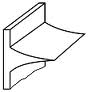
\includegraphics{ailette_parabolique}\\
%%   %\caption{倒抛物线形截面肋片}\label{ailette_parabolique}  

